\chapter{Impulse Response}\label{impulseResponseAppendix} 
\textbf{Name: Group 630}\\
\textbf{Date: 16/03 - 2016}

\subsubsection{Purpose}
To observe the impulse response of the Cubli hanging upside down.
Data is used to compare the measured response and the simulation given by the theoretical nonlinear model.

\subsubsection{Setup}
\begin{figure}[H] 
	\centering 
	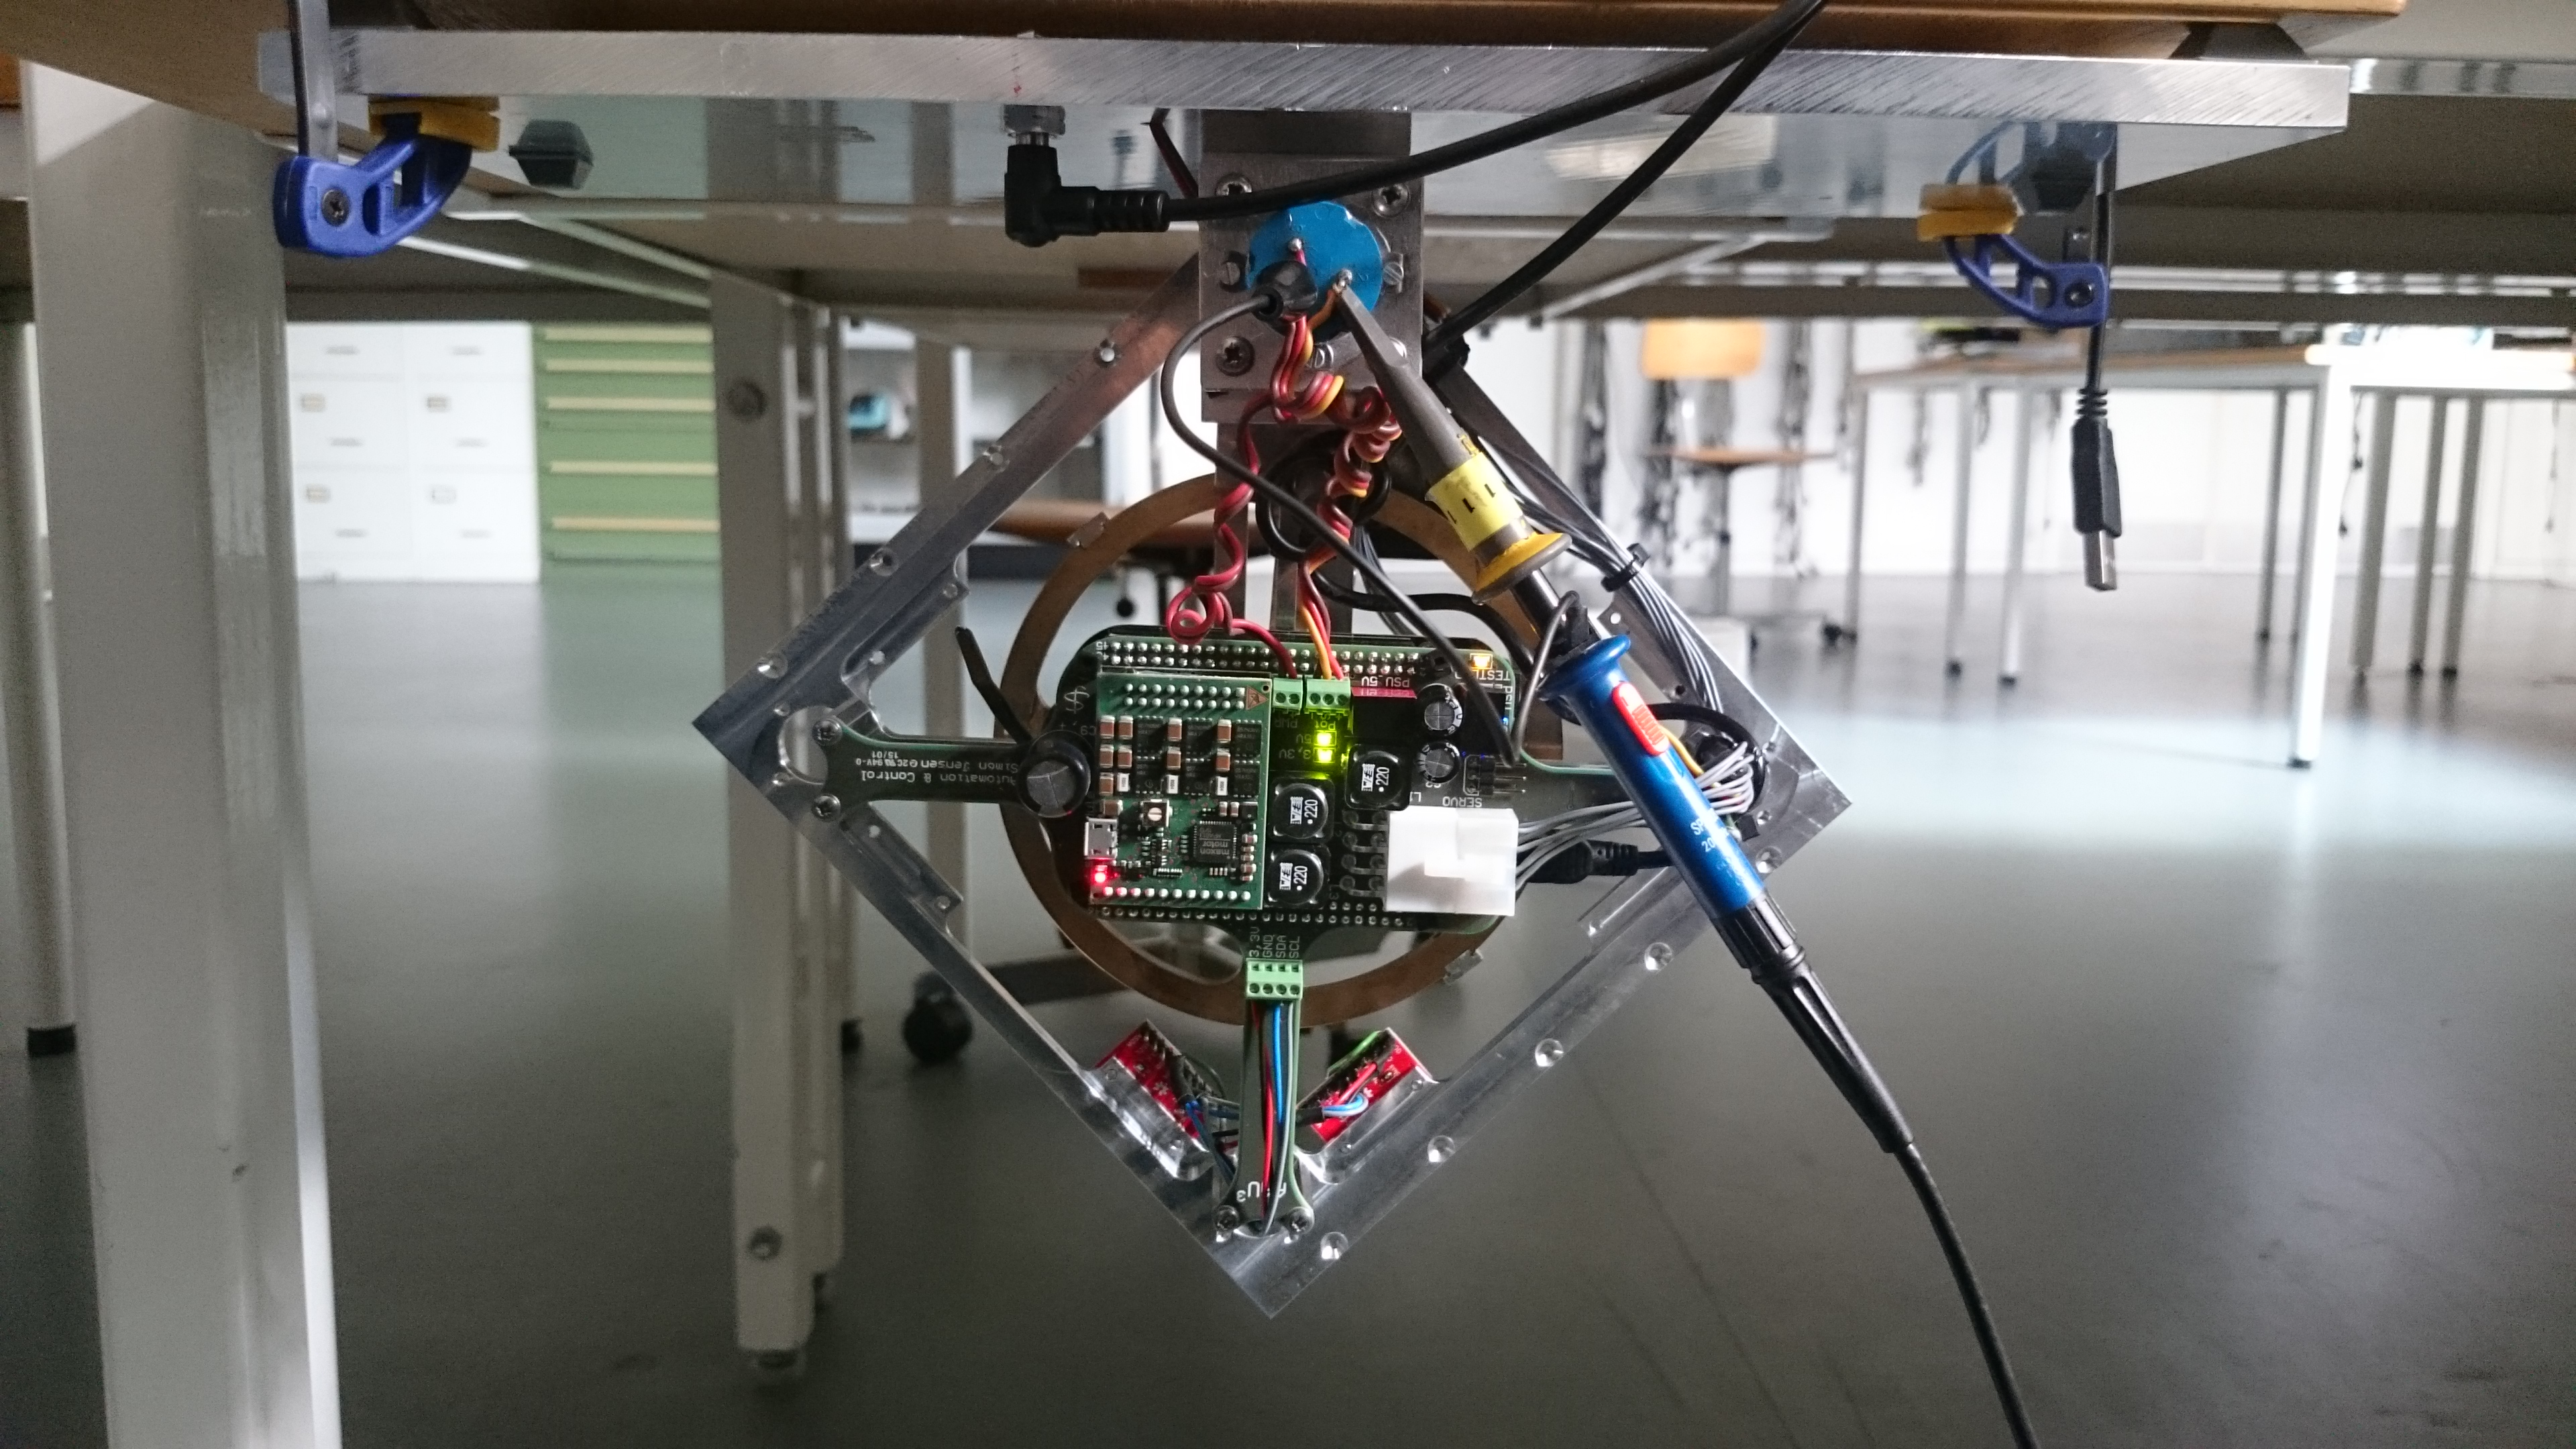
\includegraphics[scale=0.1]{figures/impulseResponseSetup}
	\caption{The Cubli setup hanging upside down beneath a table during the impulse response test}
	\label{impulseResponseTestPicture}
\end{figure} 

\subsubsection{Procedure}
\begin{enumerate}
	\item Turn on the power supply
	\item Place the setup upside-down and place the frame touching the base, \si{135^0} with respect to the vertical position
	\item Use the oscilloscope to measure the changes in the potentiometer 
	\item Let the Cubli fall
	\item Collect all the data and plot it in Matlab
	\item Compare with the simulation 	
\end{enumerate}

\subsubsection{Results}
\begin{minipage}{\linewidth}
	\begin{minipage}{0.45\linewidth}
		\begin{figure}[H]
			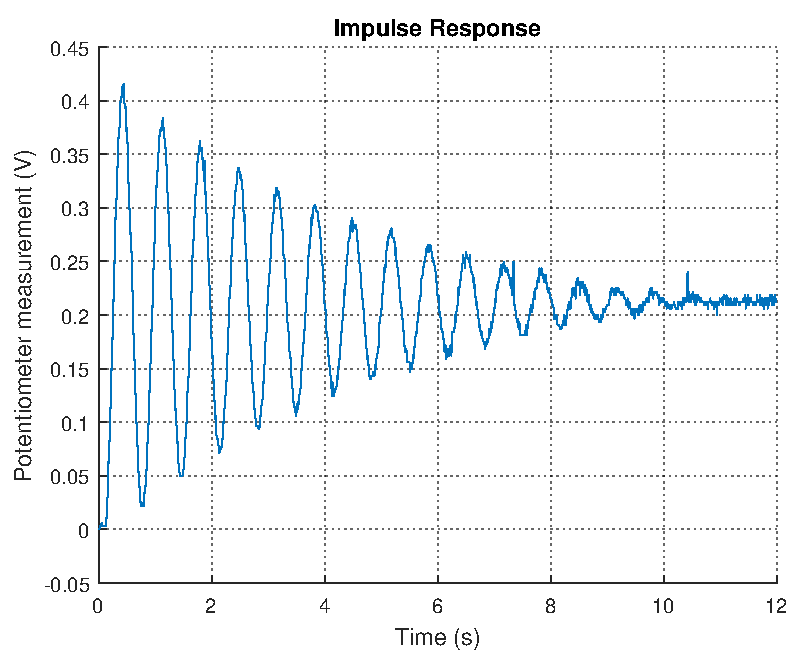
\includegraphics[scale=.53]{figures/ImpVolt}
			\centering
			\vspace{-.4cm}
			\captionsetup{justification=centering}
			\captionof{figure}{Raw data taken from the potentiometer}
			\label{ImpVolt}
		\end{figure}\vspace{-5mm}
	\end{minipage}
	\hspace{0.03\linewidth}
	\begin{minipage}{0.45\linewidth}
		\begin{figure}[H]
			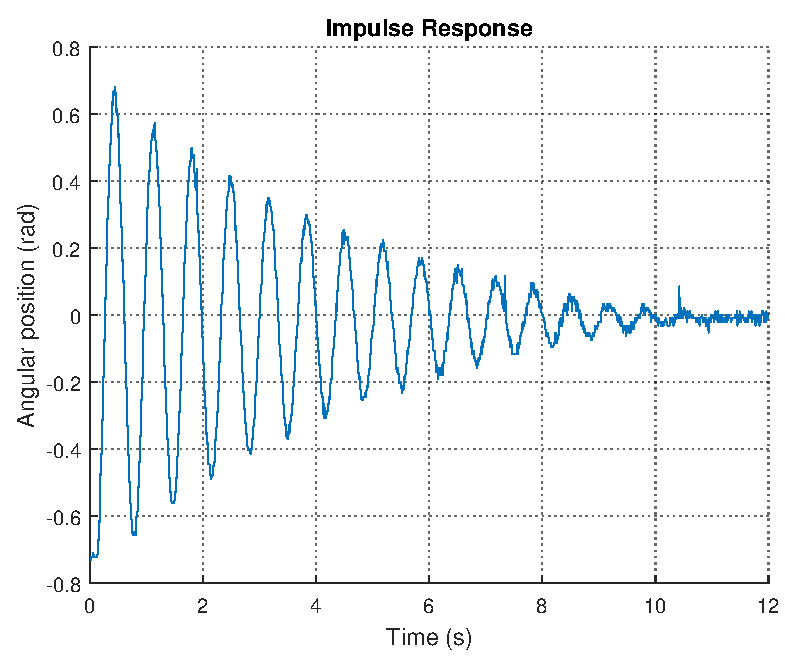
\includegraphics[scale=.53]{figures/ImpRad}
			\centering
			\vspace{-.4cm}
			\captionsetup{justification=centering}
			\captionof{figure}{Angular position of the frame}
			\label{ImpRad}
		\end{figure}\vspace{-5mm}
	\end{minipage}
\end{minipage} \fxnote{Look at the layout of picture of data placement}

The data is available as a .csv file on the CD.